\begin{figure*}[!h]
%\begin{subfigure}{0.18\linewidth}
%\centering
%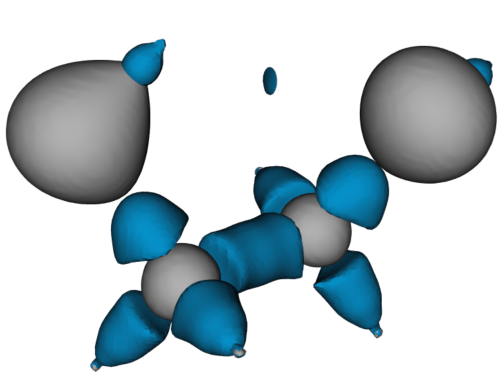
\includegraphics[width=\linewidth]{Images/EthaneDiol/gt.pdf}
%\vspace{-2mm}
%\caption{$Rho_{isoval}=1.57$ (gray),\\ $s_{isoval}=-0.575$ (light blue)}
%\label{fig:ethanediol_gt}
%\end{subfigure}
\begin{subfigure}{0.245\linewidth}
\centering
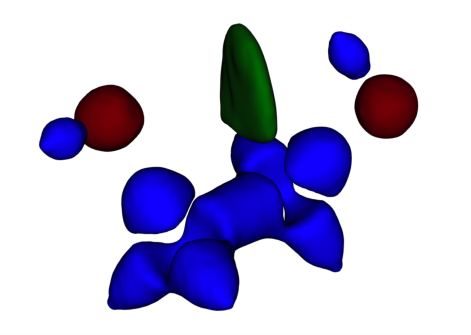
\includegraphics[width=0.95\linewidth]{Images/EthaneDiol/zls_3.pdf}
\vspace{-2mm}
\caption{$ZLS_{T}$}
\label{fig:ethanediol_zls}
\end{subfigure}
\begin{subfigure}{0.245\linewidth}
\centering
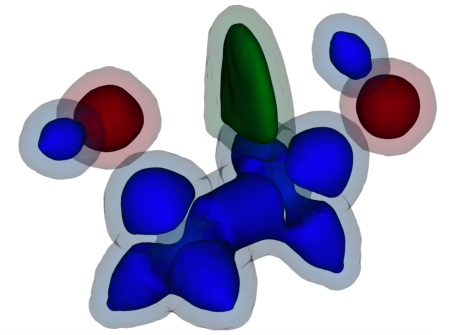
\includegraphics[width=0.95\linewidth]{Images/EthaneDiol/fls_2_3.pdf}
\vspace{-2mm}
\caption{$ZLS_{T}$ + $FLS_{T,2}$}
\label{fig:ethanediol_fls}
\end{subfigure}
\begin{subfigure}{0.245\linewidth}
\centering
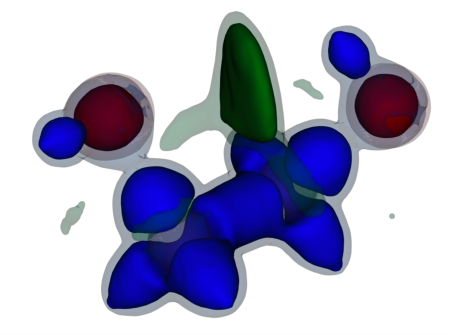
\includegraphics[width=0.95\linewidth]{Images/EthaneDiol/fcls_68_3.pdf}
\vspace{-2mm}
\caption{$ZLS_{T}$ + $FCLS_{T,68\%}$}
\label{fig:ethanediol_fcls}
\end{subfigure}
\begin{subfigure}{0.24\linewidth}
\centering
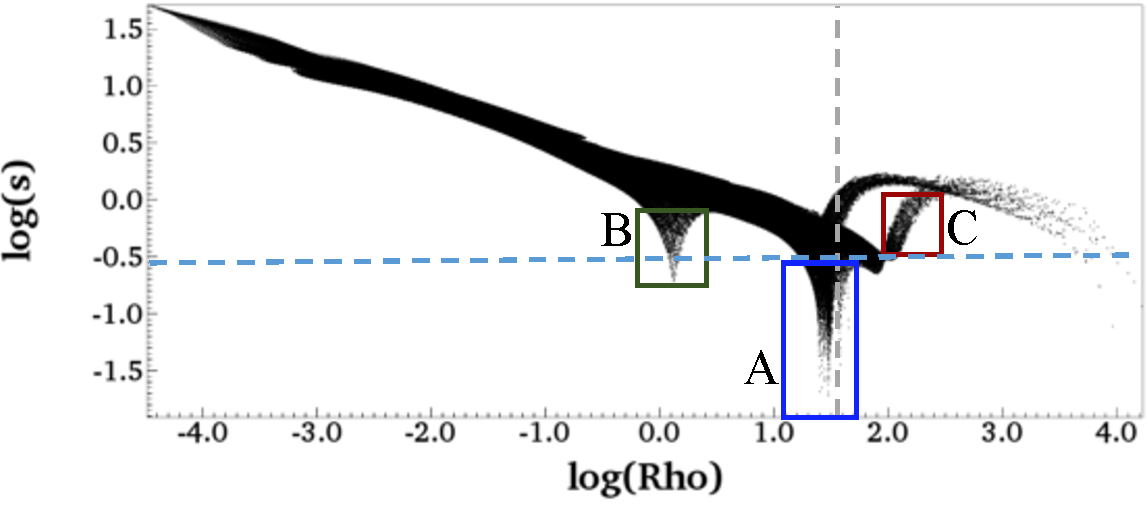
\includegraphics[width=\linewidth]{Images/EthaneDiol/scatterplot_3.pdf}
\caption{Attribute space 2D scatterplot, traits (labeled rectangular selections), and isovalues (dashed lines). We use $T = \left\{T_{A}, T_{B}, T_{C}\right\}$.\fix{continue the story} } 
\label{fig:ethanediol_scatterplot}
\end{subfigure}
\vspace{-2mm}
\caption{The covalent bonds~($T_{A}$, blue), non-covalent bond~($T_{B}$, green) and oxygen atoms~($T_{C}$, red) of an ethanediol molecule are visualized using the electron density (Rho) and reduced gradient (s) attributes.}
%\vspace{-1mm}
\label{fig:ethanediol}
\end{figure*}
